%------------------------------------ Inicio ---------------------------------------
\documentclass[11pt, a4paper]{article}

% -------------- Nombre del documento --------------
\newcommand{\nombre}{Trabajo Practico N°1}
%---------------------------------------------------------

%-------------------- Include Paquetes iniciales---------------------
\usepackage{mathtools}
\usepackage{graphicx}
\usepackage{float} 
\usepackage{geometry}
\geometry{top=35mm,bottom=30mm,left=33mm,right=33mm,headsep=15mm}
\usepackage{relsize} % agranda a un mas las letras
\usepackage[spanish,es-nodecimaldot]{babel}
\usepackage[utf8]{inputenc}
\usepackage{lastpage} % nos dice el numero total de paginas
\usepackage{fancyhdr} % modifica encabezado y pie de pagina
\pagestyle{fancy} % Con ésto aplicamos el encabezado y pie 
\renewcommand{\headrulewidth}{0.2pt} % linea encabezado tamaño
\renewcommand{\footrulewidth}{0pt} % linea pie de pagina tamaño

\cfoot{}
\pagestyle{fancy}
\fancyhf{}
\rfoot{\thepage}
\lhead{
\includegraphics[scale=0.12]{Imagenes/logounc.jpg}}
\rhead{\nombre}
%-----------------------------------------------------------------------


\begin{document}

%--------------------  Portada ---------------------


\begin{center}
	{\huge\textbf{SINTESIS DE REDES}} \\
	\vspace{3mm}
	{\huge\textbf{ACTIVAS}} \\
	\vspace{10mm}
	{\large -}
	\vspace{2mm}
	
\begin{figure}[H]
	\centering
	
\includegraphics[width=0.7\linewidth]{Imagenes/logoPrincipal.png}
\end{figure}
\vspace{10mm}
\textscale{3}{ \textbf{\nombre}} \\
\vspace{8mm}
\textscale{1.6}{ AO Ideal: Circuitos Analógicos Lineales y No Lineales\textbf{}}\\
\vspace{6mm}
	\textscale{1.3}{ Síntesis de Redes Activas - 2024\textbf{}}\\
	\vspace{15mm}
	---------------------------------------------\-\\
	\vspace{15mm}
	\textscale{1.3}{\textbf{Integrantes}}\\
	\vspace{6mm}
	\textscale{1.3}{Valentin Jose Ramirez, 43700362}\\
 \vspace{2mm}
	\textscale{1.3}{José Ignacio Lopez Sivilat, 44805902}\\
 \vspace{2mm}
	\textscale{1.3}{Franco Gabriel Lopez, 43271762} \\
     \vspace{2mm}
	\textscale{1.3}{Alejo Adrian Beierbach, 43700333} \\
	\vspace{15mm}
	\textscale{1.3}{\textbf{Profesores adjuntos}}\\
 \vspace{6mm}
 \textscale{1.3}{Dr. Ing. Pablo A. Ferreyra}\\
 \vspace{2mm}
 \textscale{1.3}{Ing. César Reale}\\
	\thispagestyle{empty}
\end{center}
\clearpage
%----------------------------fin portada-----------
\thispagestyle{empty}
\tableofcontents
\clearpage


% ------------------------------------- Desarrollo ---------------------------------
\pagenumbering{arabic}

\section{Introducción}
En este trabajo de laboratorio, se analizaran tres circuitos:
\begin{enumerate}
    \item \textbf{Circuito I:} Amplificador diferencial
    \item \textbf{Circuito II:} Fuente de Corriente Controlada por Tensión
    \item \textbf{Circuito III:} Rectificador de precisión
    \item \textbf{Circuito IV:} Comparador con histéresis
\end{enumerate}
\section{Objetivos}
Familiarizarse con el armado y análisis de circuitos analógicos lineales y no lineales. En este Trabajo Práctico debe considerar para los cálculos iniciales el amplificador como ideal. 
\section{Circuito I: Amplificador diferencial}
\begin{figure}[htb]
	\centering
	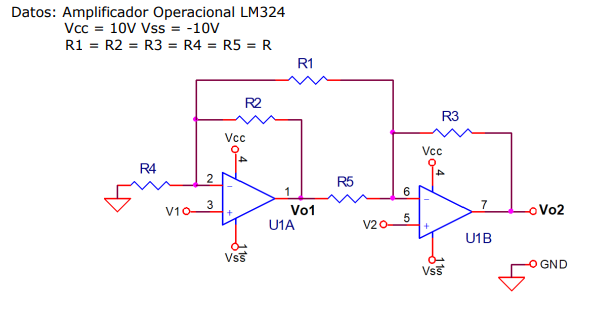
\includegraphics[width=1\textwidth]{Imagenes/circuito_consigna.png}
	\caption{Circuito propuesto}
\end{figure}
\subsection{Análisis teórico}
Se debe analizar la tensón de salida en función de la tensión de entrada en modo diferencial $ V_d=(V_2-V_1)$ y también en modo común $V_c=(V_1+V_2)/2$.\\
Para realizar el análisis en modo diferencial, se aplica el método de superposición, primero se calcula $V_{01}$ y luego $V_{02}$.
\subsubsection{Cálculo de $V_{01}$}
\onehalfspacing
\begin{flushleft}
\textbf{Pasivando $V_2$}\\
$V_{O1}|_{V_2=0}=(1+\frac{R}{R/2})V_1=3V_1$ \\
\textbf{Pasivando $V_1$} \\
$V_{O1}|_{V_1=0}=(-\frac{R}{R})V_2=-V_2$ 
\end{flushleft}\begin{center}
\boxed{\mathbf{V_{O1}=3V_1-V_2}} 	
\end{center}

\subsubsection{Cálculo de $V_{02}$}
\begin{flushleft}
\textbf{Pasivando $V_1$ y $V_2$}\\
$V_{O2}|^{V_1=0}_{V_2=0}=(-\frac{R}{R})V_1=-V_{01}$ \\
\textbf{Pasivando $V_2$ y $V_{01}$} \\
$V_{O2}|^{V_2=0}_{V_{01}=0}=(-\frac{R}{R})V_1=-V_1$ \\
\textbf{Pasivando $V_1$ y $V_{01}$} \\
$V_{O2}|^{V_1=0}_{V_{01}=0}=(1+\frac{R}{R/2})V_2=3V_2$ 
\end{flushleft}
\begin{center}
	\boxed{V_{O2}=3V_2-V_1-3V_1+V_2=4V_2-4V_1=4(V_2-V_1)}\\
	reemplazando con $ V_d=(V_2-V_1)$ \\
    \boxed{\mathbf{V_{O2}} = 4V_d}
\end{center}
\begin{flushleft}
	Para el análisis en $V_c=(V_1+V_2)/2$ y haciendo $V_1=V_2$ tenemos que \begin{center}
		\boxed{\mathbf{V_{02}=0}}
	\end{center}
\end{flushleft}
\subsubsection{Impedancias}
Las impedancias vistas por las fuentes de señales $V_1$ y $V_2$ son las impedancias de entrada de ambos amplificadores. Definimos $Z_{i1}$ y $Z_{i2}$ a las impedancias vistas por $V_1$ y $V_2$ respectivamente.
\begin{center}
	$Z_{i1}= \frac{V_1}{I_{i1}}$ al ser $I_{i1}=0$ \\
	entonces queda $Z_{i1}= \infty$\\
	de igual forma se determina que\\
	 $Z_{i2}=\frac{V_2}{I_{i2}}=\infty$
\end{center}
\subsection{Simulaciones en LTSpice}
Se realizaron diferentes simulaciones con LTSpice para observar en la practica la veracidad de las ecuaciones correspondientes a las salidas dependiendo el modo del amplificador, tanto en modo común como en modo diferencial. A continuación se listan las simulaciones realizadas:
\begin{itemize}
	\item $Vo_1$ y $Vo_2$ con $V_1=0.5[V]$ y $V_2=1[V]$.
	\item $Vo_1$ y $Vo_2$ con $V_1=1[V]$ y $V_2=1[V]$.
\end{itemize}
\begin{figure}[H]
	\centering
	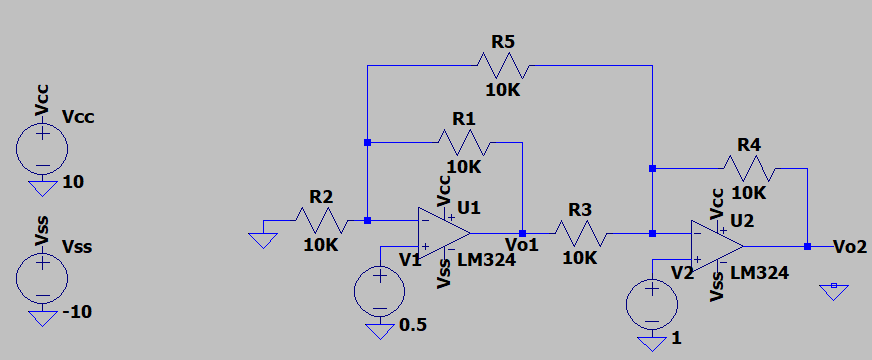
\includegraphics[width=1\textwidth]{Imagenes/Circuito1_1.png}
	\caption{Circuito simulado}
\end{figure}
\begin{figure}[H]
	\centering
	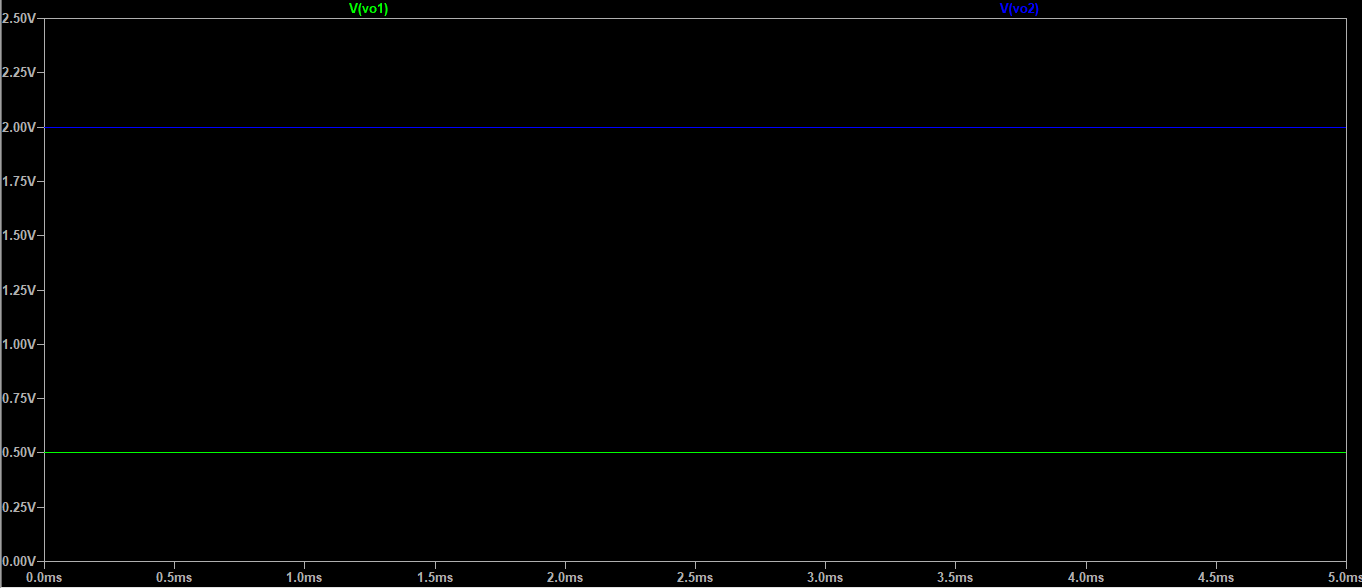
\includegraphics[width=1\textwidth]{Imagenes/Sim1.png}
	\caption{$Vo_1$ (verde) y $Vo_2$ (azul) con $V_1=0.5[V]$ y $V_2=1[V]$.}
\end{figure}
\begin{figure}[H]
	\centering
	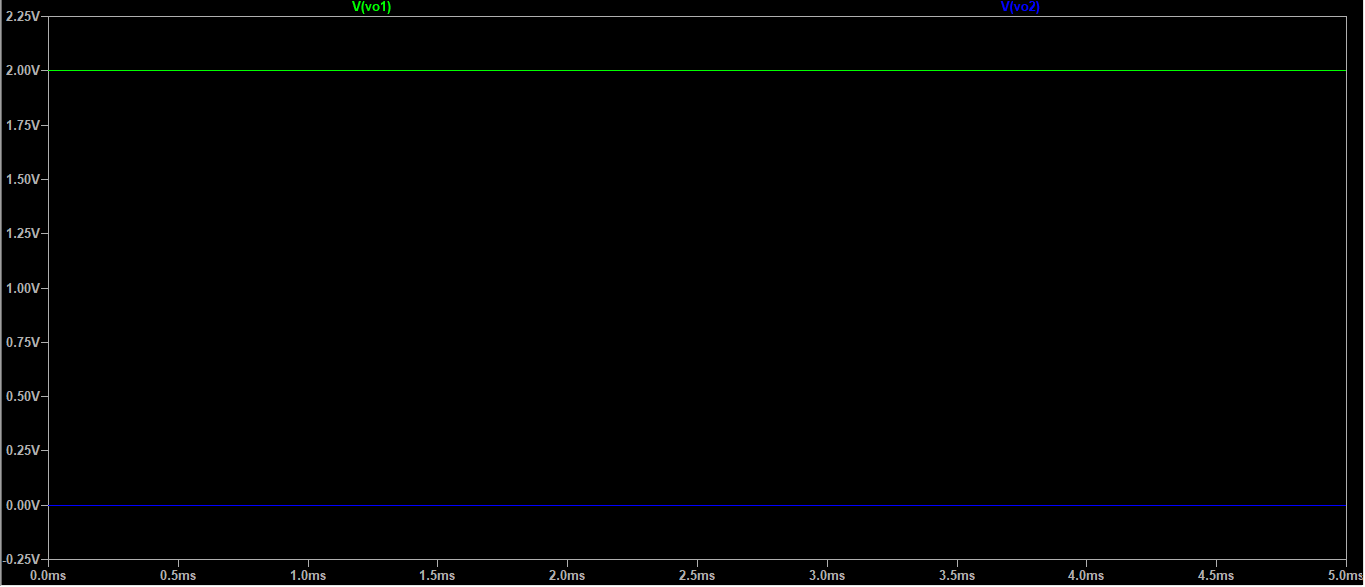
\includegraphics[width=1\textwidth]{Imagenes/Sim2.png}
	\caption{$Vo_1$ (verde) y $Vo_2$ (azul) con $V_1=1[V]$ y $V_2=1[V]$.}
\end{figure}

\section{Circuito II: Fuente de Corriente Controlada por Tensión}
\begin{figure}[htb]
	\centering
	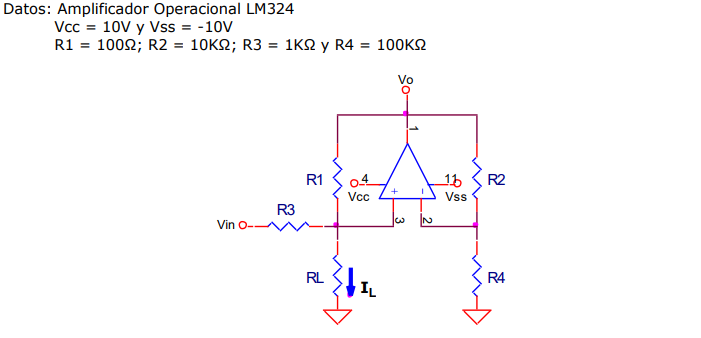
\includegraphics[width=1\textwidth]{Imagenes/Circ2.png}
	\caption{Circuito propuesto}
\end{figure}
\subsection{Análisis teórico}
Para analizar el circuito propuesto, se propone expresar $V^+$ (la entrada no inversora del AO) y $V^-$ (la entrada inversora del AO) en función del Vo, planteando el divisor resistivo en el nodo "2" de la figura:
\begin{center}
	$V^+ = V^- = V_o \frac{R_4}{R_4 + R_2}$
\end{center}
luego se plantea la ley de los nodos de Kirchhoff en el nodo "3"
\begin{center}
	$\frac{V_{in} - V^+ }{R_3} + \frac{V_o - V^+ }{R_1} = \frac{V^+}{R_L}$
\end{center}
\begin{center}
	$\frac{V_{in}}{R_3} + \frac{V_o}{R_1} = V^+ (\frac{1}{R_L} + \frac{1}{R_1} + \frac{1}{R_3})$
\end{center}
y reemplazando $V^+$
\begin{center}
	$\frac{V_{in}}{R_3} + \frac{V_o}{R_1} = V_o \frac{R_4}{R_4 + R_2} (\frac{1}{R_L} + \frac{1}{R_1} + \frac{1}{R_3})$
\end{center}
\begin{center}
	$V_{in} = V_o[\frac{1}{R_L}( R_3 \frac{R_4}{R_4 + R_2}) + (R_3 \frac{R_4}{R_4 + R_2}) (\frac{1}{R_1} + \frac{1}{R_3} ) - \frac{R_3}{R_1}]$
\end{center}
Reemplazando para $R_1=100[\Omega]$, $R_2=10[K\Omega]$, $R_3=1[K\Omega]$ y $R_4=100[K\Omega]$:
\begin{center}
	$V_{in} = V_o[\frac{1}{R_L}(909.09091)]$
\end{center}
Luego la corriente que circula por la carga se define:
\begin{center}
	$I_{RL} = \frac{V^+}{R_L}$
\end{center}
\begin{center}
	$I_{RL} = V_o \frac{R_4}{R_4 + R_2} \frac{1}{R_L}$
\end{center}
\begin{center}
	$I_{RL} = \frac{V_{in}}{[\frac{1}{R_L}( R_3 \frac{R_4}{R_4 + R_2}) + (R_3 \frac{R_4}{R_4 + R_2}) (\frac{1}{R_1} + \frac{1}{R_3} ) - \frac{R_3}{R_1}]} \frac{R_4}{R_4 + R_2} \frac{1}{R_L}$
\end{center}
\begin{center}
	$I_{RL} = \frac{V_{in}}{R_3}$
\end{center}
\begin{center}
	\boxed{I_{RL} = V_{in} 10^{-3}} 
\end{center}
de igual manera se define la tensión $V_o$ en función de $R_L$ y de $V_{in}$
\begin{center}
	$V_o = \frac{V_{in}}{(\frac{1}{R_L} (909.09091))}$
\end{center}
\begin{center}
	\boxed{V_o = V_{in} R_L (1.1 *10^{-3})} 
\end{center}
Por último, se determina el valor de $R_{Lmax}$ teniendo en cuenta que al ser ideal el A.O. la tensión de salida máxima será la misma que $V_{cc} = 10[V]$. Por lo tanto operando se obtiene:
\begin{center}
	\boxed{R_{Lmax} = \frac{9090}{V_{in}}} 
\end{center}
A partir de las relaciones obtenidas, se procede a completar la siguiente tabla:
\begin{table}[H]
	\begin{center}
		\begin{tabular}{| c | c | c | c | c |}
			\hline
			\multicolumn{2}{ |c| }{-} &
			\multicolumn{3}{ |c| }{$V_{in}$[V]} \\ \hline
			
			\multicolumn{2}{ |c| }{$I_{RL}$[\textmu A]} & 0.5 & 1 & 2 \\ \hline
			\multirow{5}{*}{$R_L$[K$\Omega$]}	&  0 &   0 &    0  &   0 \\
			&  1 & 500 & 1000 & 2000 \\
			&  2 & 500 & 1000 & 2000 \\
			&  5 & 500 & 1000 & 2000 \\
			& 10 & 500 & 1000 & 2000 \\ \hline
	
		\end{tabular}
				\caption{Valores teóricos de $I_{RL}$ en función de $R_L$ y de $V_{in}$}
		\end{center}
\end{table} 

\begin{table}[H]
	\begin{center}
		\begin{tabular}{| c | c | c | c | c |}
			\hline
			\multicolumn{2}{ |c| }{-} &
			\multicolumn{3}{ |c| }{$V_{in}$[V]} \\ \hline
			
			\multicolumn{2}{ |c| }{$V_o$[V]} & 0.5 & 1 & 2 \\ \hline
			\multirow{5}{*}{$R_L$[K$\Omega$]} & 0	& 0    & 0   & 0   \\
			& 1	& 0.55 & 1.1 & 2.2 \\
			& 2	& 1.1  & 2.2 & 4.4 \\
			& 5	& 2.75 & 5.5 & 11  \\
			& 10	& 5.5  & 11  & 22  \\ \hline
			
		\end{tabular}
		\caption{Valores teóricos de $V_o$ en función de $R_L$ y de $V_{in}$}
	\end{center}
\end{table} 
Aquellos valores que superen el valor de la tensión de $V_{cc}$, la salida se enclava a ese mismo valor y la forma de la onda se recorta.

\subsection{Simulaciones}
Realizamos diferentes simulaciones con LTSpice para lograr observar el comportamiento de $I_{RL}$ y $V_o$. 
\begin{figure}[H]
	\centering
	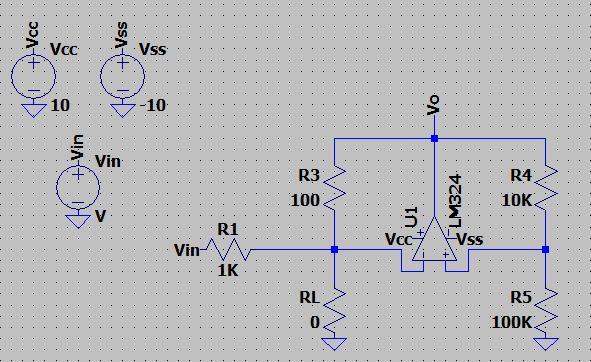
\includegraphics[width=1\textwidth]{Imagenes/Sim3.png}
	\caption{Circuito simulado}
\end{figure}
\begin{figure}[H]
	\centering
	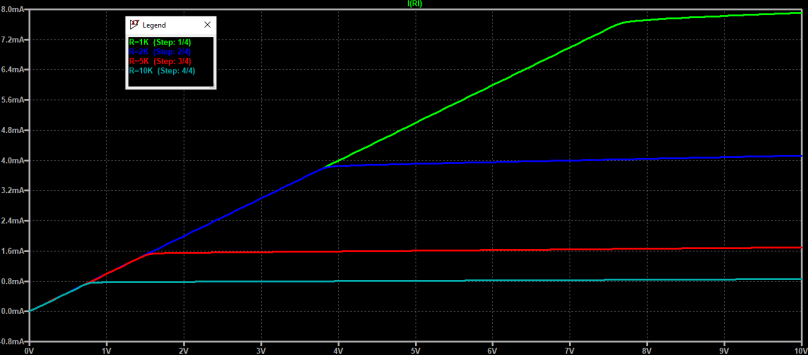
\includegraphics[width=1\textwidth]{Imagenes/IlvsVin.png}
    \caption{$I_{RL} = f(R_L , V_{in})$}
\end{figure}
Para la primer simulación se hizo un barrido en continua de 0[V] a 10[V], ya que desde -10[V] la respuesta es muy similar. En esta, podemos ver cómo la variación de la corriente es lineal hasta el punto de tensión para cada valor de $R_L$  que satura al operacional. 
\begin{center}
	\begin{tabular}{| c | c |}
		\hline
		      $R_L$     &   $V_{in-sat}$ \\ \hline
		 1 [K$\Omega$] 	&   	7.6 [V]	 \\
		 2 [K$\Omega$] 	&  	    3.8 [V]	 \\
		 5 [K$\Omega$] 	&    	1.5 [V]	 \\
		10 [K$\Omega$] 	&   	0.7 [V]	 \\ \hline
	\end{tabular}
	\begin{figure}[H]
		\centering
		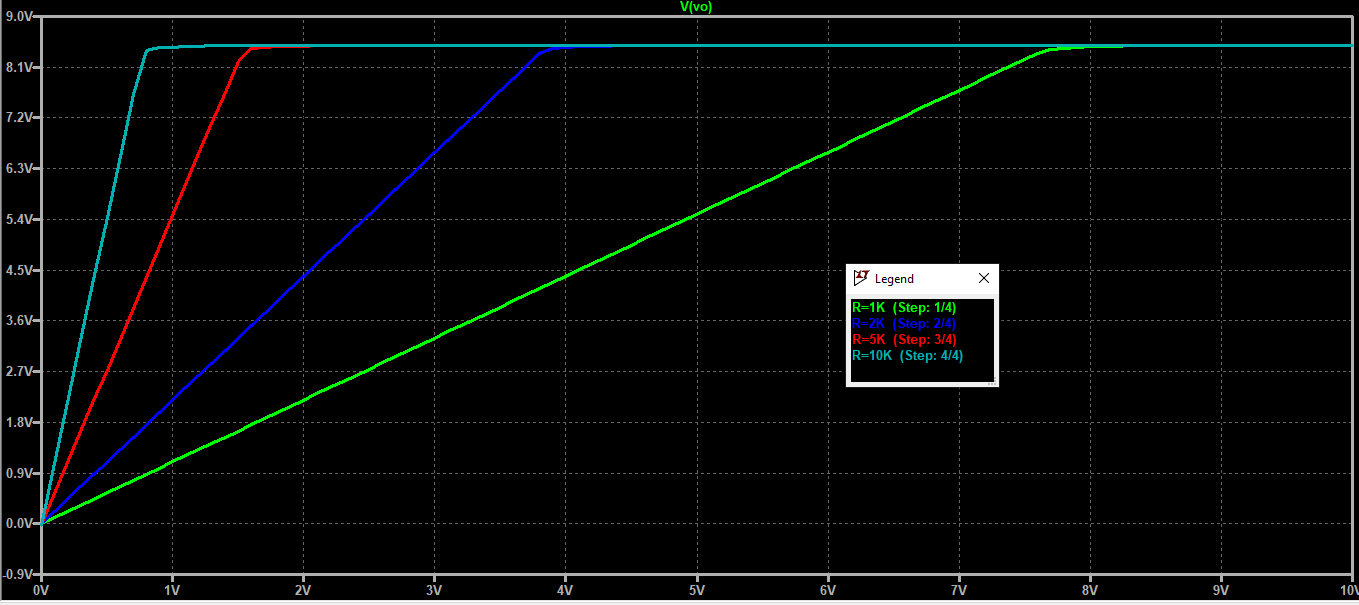
\includegraphics[width=1\textwidth]{Imagenes/vo_vin.png}
		\caption{$V_o = f(V_{in}, R_L)$}
	\end{figure}
\end{center} 
Finalmente, en el cuadro se puede ver cómo afectan la tensión de entrada y los valores de $R_L$ propuestos a la tensión de salida.

\begin{table}[H]
	\begin{center}
		\begin{tabular}{| c | c | c | c | c |}
			\hline
			\multicolumn{2}{ |c| }{-} &
			\multicolumn{3}{ |c| }{$V_{in}$[V]} \\ \hline
			
			\multicolumn{2}{ |c| }{$I_{RL}$[\textmu A]} 
									 & 0.5    & 1 	   &    2 \\ \hline
			
	\multirow{$R_L$[K$\Omega$]} 	&  0 &   0    &   0    &    0 \\
				&  1 & 495 & 994 & 1995 \\
				&  2 & 495 & 993 & 1990 \\
				&  5 & 493 & 990 & 1549 \\
				& 10 & 488 & 771 &  783 \\ \hline
			
		\end{tabular}
		\caption{Valores simulados de $I_{RL}$ en función de $R_L$ y de $V_{in}$}
	\end{center}
\end{table} 
\newpage
\section{Circuito III: Rectificador de Precisión}
\onehalfspacing
\begin{figure}[htb]
	\centering
	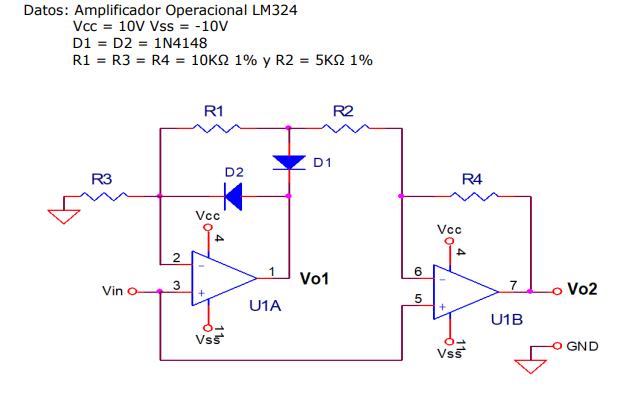
\includegraphics[width=1\textwidth]{Imagenes/Circuito3_consigna.png}
	\caption{Circuito propuesto}
\end{figure}
En este circuito se tienen 2 AO LM324 con diodos trabajando como un rectificador de precisión con una señal común para ambos. La fuente de alimentación es simétrica en +/- 10[V]. Los diodos utilizados son 1N4148.
\subsection{Análisis teórico}
Para determinar $V_o$ en función de $V_{in}$ el análisis se hace para cuando $V_{in}$ es positiva y cuando $V_{in}$ es negativa.
\subsubsection{$V_o = f(V_{in})$ con $V_{in}$ $> 0$  }
Para ésta condición entonces D2 = ON y D1= OFF. \\
Además considerando pasivada la entrada del AO U1B se plantea la ley de los nodos de Kirchhoff en el nodo "6"
\begin{center}
	$\frac{V_o}{R_4} = - \frac{V_{in}}{R_1 + R_2}$
\end{center}
\begin{center}
	$\frac{V_o}{10[K\Omega]} = - \frac{V_{in}}{15[K\Omega]}$
\end{center}
\begin{center}
	$V_o= - \frac{2}{3} V_{in}$
\end{center}
Luego pasivando la entrada de U1A
\begin{center}
	$V_{in}= V_o \frac{R_1 + R_2}{R_1 + R_2 + R_4}$
\end{center}
\begin{center}
	$V_{in}= V_o \frac{15[K\Omega]}{25[K\Omega]}$
\end{center}
\begin{center}
	$V_o = \frac{5}{3} V_{in}$
\end{center}
Aplicando superposición para encontrar el resultado completo
\begin{center}
	$V_o = V_{in} \frac{5}{3} - V_{in} \frac{2}{3}$
\end{center}
\begin{center}
	\boxed{V_o = V_{in} }
\end{center}

\subsubsection{$V_o = f(V_{in})$ con $V_{in}$ $< 0$  }
Para ésta condición entonces D1 = ON y D2= OFF. \\
Además considerando pasivada la salida del AO U1A se plantea la ley de los nodos de Kirchhoff en el nodo "6"
\begin{center}
	$V_{in} = V_o \frac{R_2}{R_2 + R_4}$
\end{center}
\begin{center}
	$V_{in} = V_o \frac{5[K\Omega]}{15[K\Omega]}$
\end{center}
\begin{center}
	$V_o= 3 V_{in}$
\end{center}
Luego pasivando la entrada de U1B y tomando $V_{oB}$ como tensión de salida del amplificador U1B, resulta:
\begin{center}
	$\frac{V_{oB}}{R_2} =- \frac{V_o}{R_4}$
\end{center}
\begin{center}
	$\frac{V_{oB}}{5[K\Omega]} =- \frac{V_o}{10K\Omega}$
\end{center}
\begin{center}
	$V_o = -2 V_{oB} $
\end{center}
Por otro lado, la tensión de salida de $V_{oB}$ se obtiene planteando el divisor de tension del AO U1B:
\begin{center}
	$V_{in} = V_{oB} \frac{R_3}{R_1 + R_3}$
\end{center}
\begin{center}
	$V_{in} = V_{oB} \frac{10K\Omega}{20K\Omega}$
\end{center}
\begin{center}
	$V_{in} =\frac{1}{2} V_{oB} $
\end{center}
Reemplazando queda:
\begin{center}
	$V_o = -4 V_{in} $
\end{center}
Aplicando superposición para encontrar el resultado completo
\begin{center}
	$V_o = 3 V_{in} - 4 V_{in}$
\end{center}
\begin{center}
	\boxed{V_o = - V_{in} }
\end{center}
Entonces, cuando la tensión de entrada es positiva, la tensión de salida es igual a la entrada, mientras que cuando la tensión de entrada es negativa, la tensión de salida tendrá la misma amplitud, pero será positiva.
\newpage
\subsection{Simulación}
\begin{figure}[htb]
	\centering
	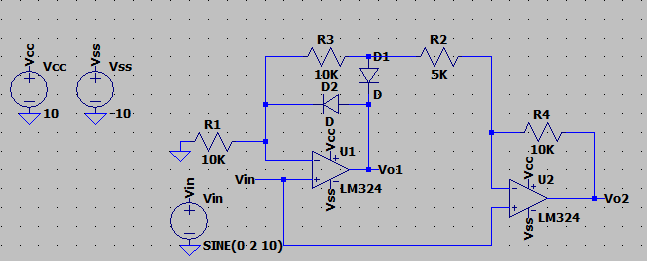
\includegraphics[width=1\textwidth]{Imagenes/Sim4.png}
	\caption{Circuito propuesto}
\end{figure}
Para observar el comportamiento de la tensión de salida del primer y segundo amplificador, utilizamos una señal senoidal sin offset, de amplitud 2 V y con una frecuencia de 10 Hz. La amplitud de la señal sera variada en distintas simulaciones para ver el efecto que produce en la rectificación y encontrar los limites de la misma.
\begin{figure}[H]
	\centering
	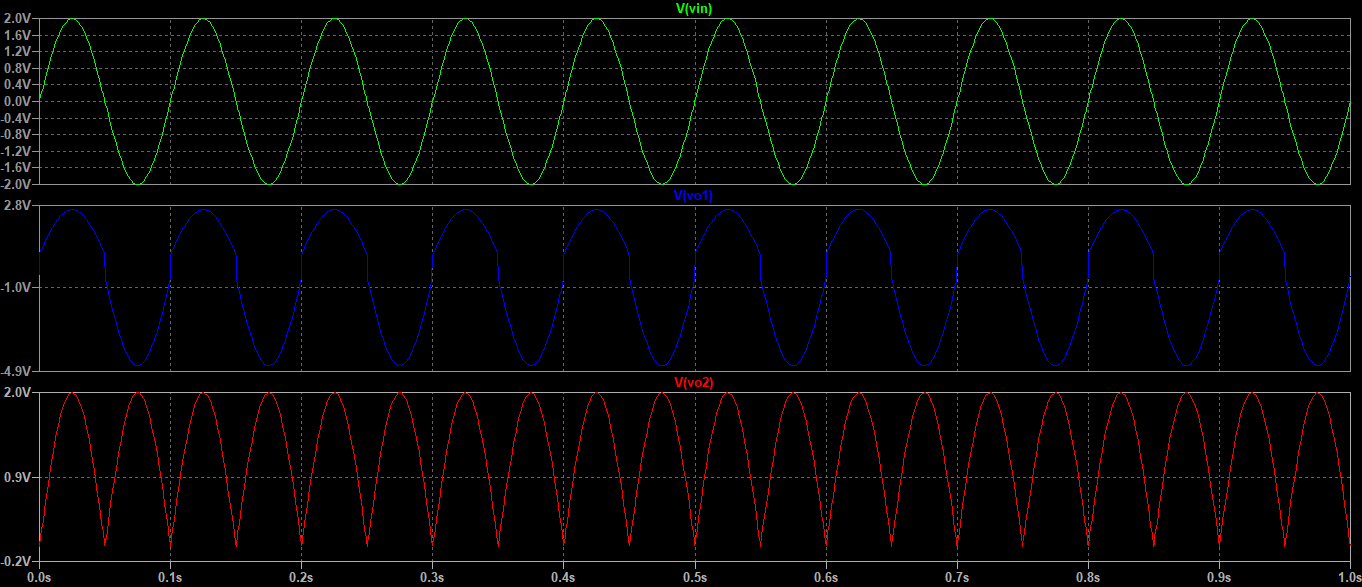
\includegraphics[width=1\textwidth]{Imagenes/Vin2V.png}
	\caption{$Vo_1$ (azul) y $Vo_2$ (rojo) con $V_{in}=2[V]$ (verde).}
\end{figure}
\begin{figure}[H]
	\centering
	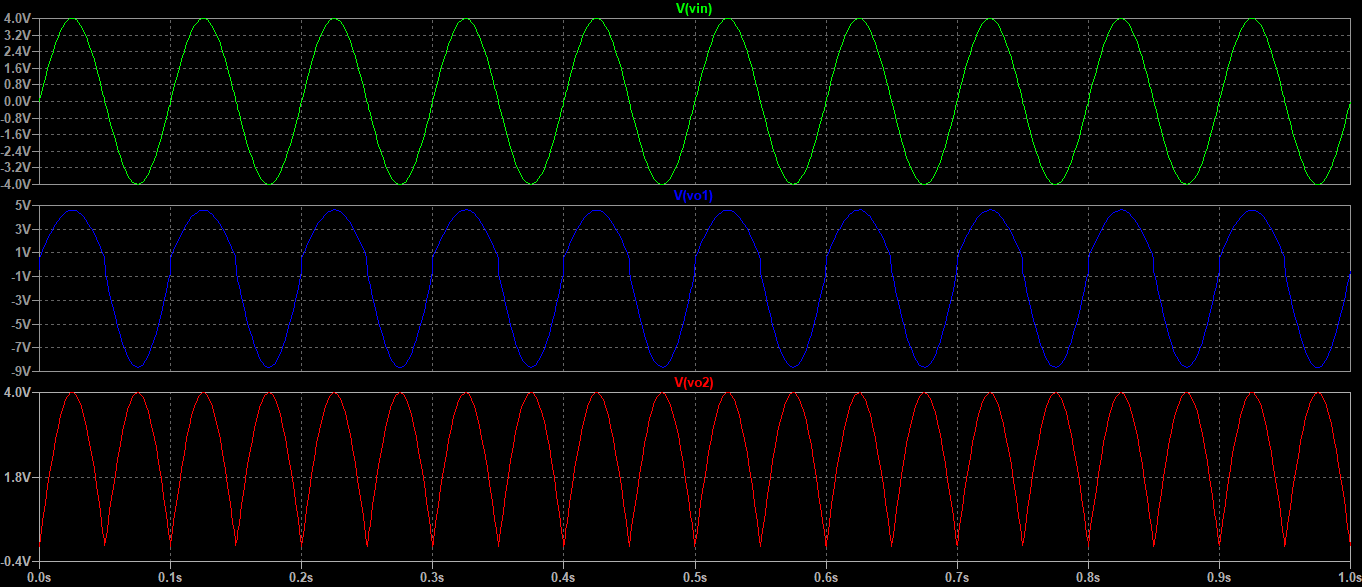
\includegraphics[width=1\textwidth]{Imagenes/Vin4v.png}
	\caption{$Vo_1$ (azul) y $Vo_2$ (rojo) con $V_{in}=4[V]$ (verde).}
\end{figure}
\begin{figure}[H]
	\centering
	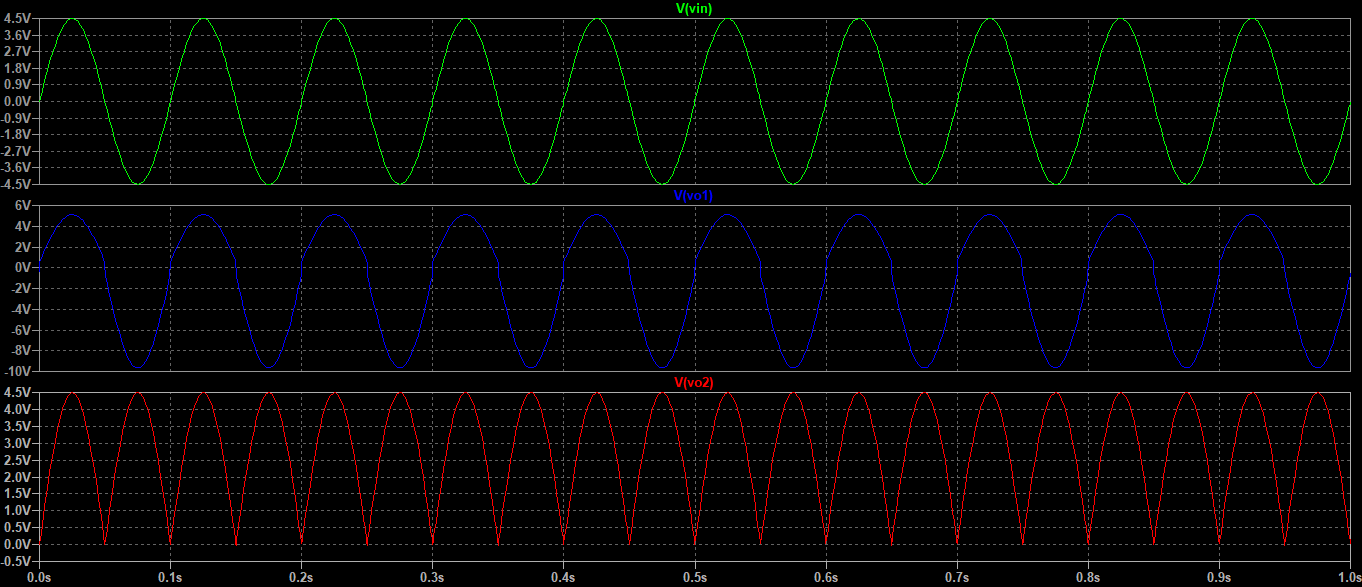
\includegraphics[width=1\textwidth]{Imagenes/Vin4.5LimiteSat.png}
	\caption{$Vo_1$ (azul) y $Vo_2$ (rojo) con $V_{in}=4.5[V]$ (verde). Este es el limite de saturación de la salida del primer amplificador.}
\end{figure}
\begin{figure}[H]
	\centering
	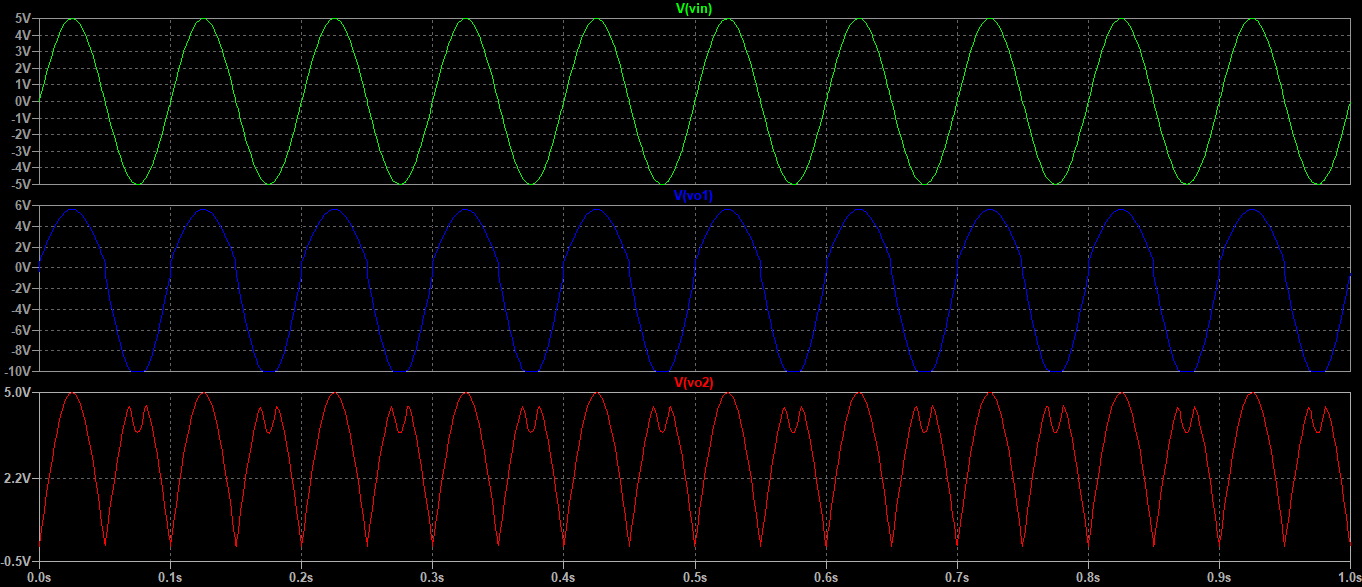
\includegraphics[width=1\textwidth]{Imagenes/Vin5v.png}
	\caption{$Vo_1$ (azul) y $Vo_2$ (rojo) con $V_{in}=5[V]$. La rectificación de la señal se ve distorsionada por la saturación del primer amplificador.}
\end{figure}
\begin{figure}[H]
	\centering
	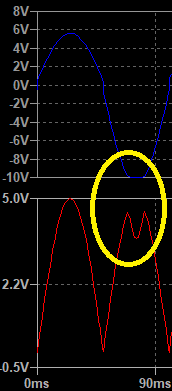
\includegraphics[width=0.3\textwidth]{Imagenes/Saturacionzoom.png}
	\caption{$Vo_1$ (azul) y $Vo_2$ (rojo) con $V_{in}=5[V]$. Aquí podemos ver como la salida del primer amplificador se satura en la parte negativa, distorsionando la rectificación de la señal.}
\end{figure}
Podemos ver entonces como el rectificador funciona perfectamente dentro del rango de -4.5 [V] y 4.5[V]. Sin embargo para valores fuera de ese rango, la salida comienza a distorsionarse debido a que la salida del primer AO comienza a saturarse debido a las alinealidades nombradas anteriormente.

\section{Circuito IV: COMPARADOR CON HISTÉRISIS}
\begin{figure}[htb]
	\centering
	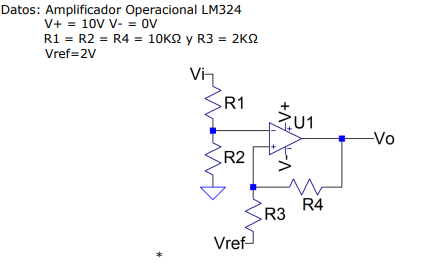
\includegraphics[width=1\textwidth]{Imagenes/circuito4.png}
	\caption{Circuito propuesto}
\end{figure}
\subsection{Análisis teórico}
Para un análisis mas detallado se considera el caso general con alimentación simétrica y que el A.O. no sea del tipo Rail to Rail. Se analiza $V_o$ a partir de la tensión diferencial $V_d$ y por último se analiza el caso particular con $V_{ss}=0$.\\
Se definen $v^+$ y $v^-$ de la siguiente manera:
\begin{center}
	$v^- = k_1 * V_{in}$
\end{center}
\begin{center}
	$v^+ = k_2 * (V_o - V_{ref})+V_{ref}$
\end{center}
teniendo que:
\begin{center}
	$k_1 = \frac{R_2}{R_1 + R_2}$
\end{center}
\begin{center}
	$k_2 = \frac{R_3}{R_3 + R_4}$
\end{center}

\subsubsection{Si $V_d<0$}
Para un A.O ideal si $V_d<0$ la salida del amplificador debería ser $V_{ss}$
\begin{center}
	
	$V_d = (v^+ - v^-)<0 \rightarrow  V_o = V_{ss}$
\end{center}
entonces
\begin{center}
	$v^+ < v^-$
\end{center}
\begin{center}
	$k_2 * (v_o - v_{ref})+ v_{ref} < k_1 * v_{in}$
\end{center}
\begin{center}
	$\frac{k_2}{k_1} * (v_o- v_{ref}) + \frac{v_{ref}}{k_1} <v_{in}$ 
\end{center}
\begin{center}
	$\frac{k_2}{k_1} * v_o + \frac{1 - k_2}{k_1} * v_{ref} <v_{in}$ 
\end{center}

\begin{center}
	$\left\{\begin{matrix}
	v_o = v_{cc}\\ 
	v_{cc} = 10[V]\\ 
	v_{ref} = 2[V]\\ 
	R_3 = 2[K\Omega]\\ 
	R_1 = R_2 = R_3 = 10[K\Omega]
\end{matrix}\right.$
\end{center}
\begin{center}
	$v_{in} > 6.67[V] \rightarrow v_o = v_{ss}$ 
\end{center}

\subsubsection{Si $V_d>0$}
Para un A.O ideal si $V_d>0$ la salida del amplificador debería ser $V_{cc}$
\begin{center}
	
	$V_d = (v^+ - v^-)>0 \rightarrow  V_o = V_{cc}$
\end{center}
entonces
\begin{center}
	$v^+ > v^-$
\end{center}
\begin{center}
	$k_2 * (v_o - v_{ref})+ v_{ref} > k_1 * v_{in}$
\end{center}
\begin{center}
	$\frac{k_2}{k_1} * (v_o- v_{ref}) + \frac{v_{ref}}{k_1} > v_{in}$ 
\end{center}
\begin{center}
	$\frac{k_2}{k_1} * v_o + \frac{1 - k_2}{k_1} * v_{ref} > v_{in}$ 
\end{center}

\begin{center}
	$\left\{\begin{matrix}
		v_o = v_{ss}\\ 
		v_{ss} = -10[V]\\ 
		v_{ref} = 2[V]\\ 
		R_3 = 2[K\Omega]\\ 
		R_1 = R_2 = R_3 = 10[K\Omega]
	\end{matrix}\right.$
\end{center}
\begin{center}
	$v_{in} < 0[V] \rightarrow v_o = v_{cc}$ 
\end{center}
resumiendo entonces lo obtenido:
\begin{center}
	$v_o(v_{in}) = \left\{\begin{matrix}
		v_{cc}$ para $v_{in} < 0[V]\\ 
		v_{ss}$ para $v_{in} > 6.67[V]
	\end{matrix}\right.$
\end{center}
\subsubsection{Si $V_{ss} = 0$}
Para este caso particular la relación queda 
\begin{center}
	$\frac{1 - k_2}{k_1} * v_{ref} > v_{in}$
\end{center}
donde se ve que el punto de conmutación queda directamente dependiente de $v_{ref}$.
\begin{center}
	Reemplazando $\left\{\begin{matrix}
		v_{ref} = 2[V] \\
		R_3 = 2[K\Omega] \\
		R_1 = R_2 = R_4 10[K\Omega]
	\end{matrix}\right.$
\end{center}
\begin{center}
 Si: $v_{in} < 3.33[V] \rightarrow v_o = v_{ss}$
\end{center}
Los análisis anteriores son válidos para un amplificador ideal o de tipo Rail to Rail, en este caso obtenido por simulación la salida máxima del LM324 es de 8.5[V], entonces queda:
\begin{center}
	Si: $v_{in} > 6.17[V] \rightarrow v_o = v_{cc}$
\end{center}
Finalmente para el LM324 y $v_{ss}=0$
\begin{center}
	$v_o(v_{in}) = \left\{\begin{matrix}
		v_{cc}$ para $v_{in} < 3.33[V]\\ 
		v_{ss}$ para $v_{in} > 6.77[V]
	\end{matrix}\right.$
\end{center}
\subsection{Simulación}
\begin{figure}[H]
	\centering
	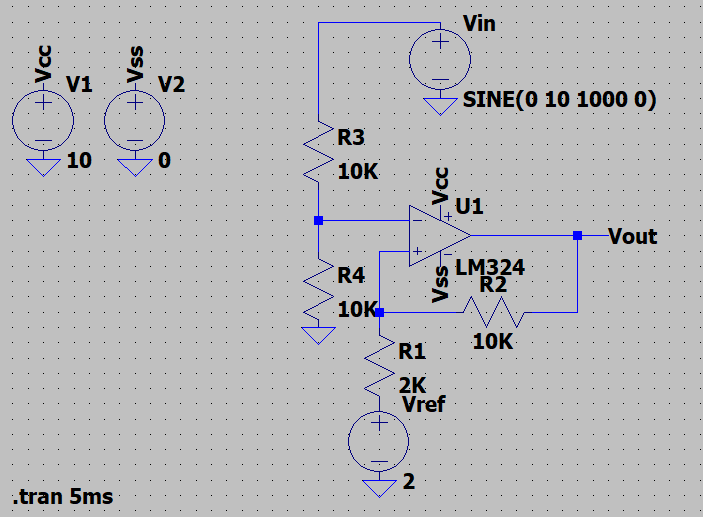
\includegraphics[width=1\textwidth]{Imagenes/Circuito4Sim.png}
	\caption{Circuito simulado}
\end{figure}
\begin{figure}[H]
	\centering
	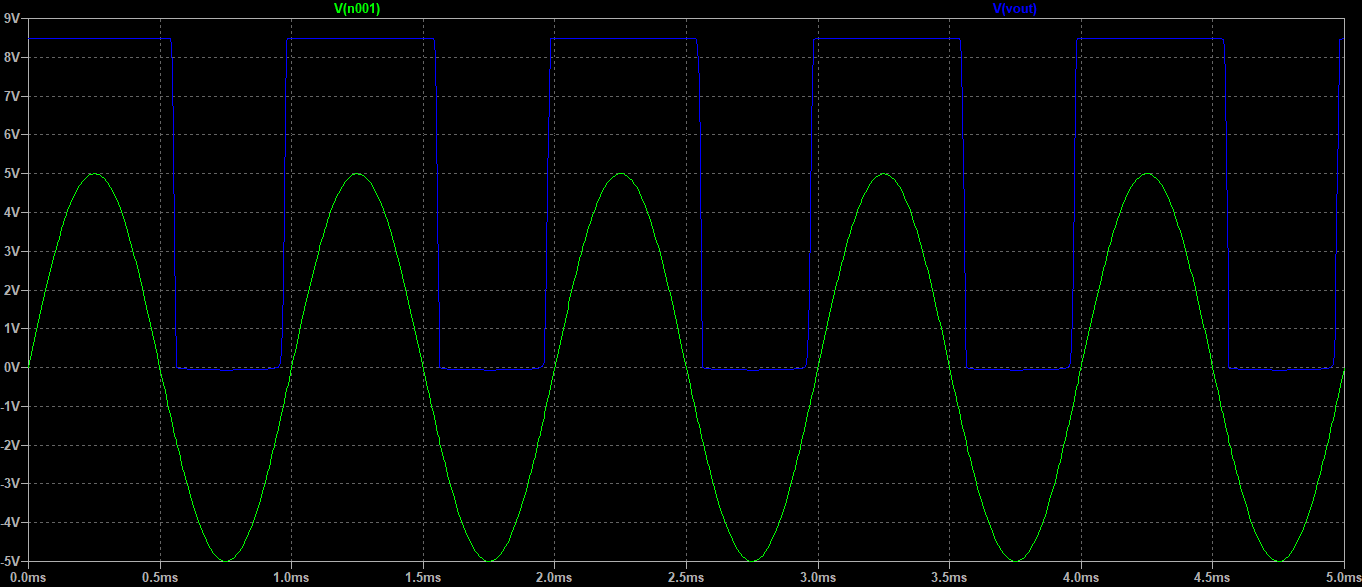
\includegraphics[width=1\textwidth]{Imagenes/ComparadorConHisteresis.png}
	\caption{$Vo_1= f(v_{in})$ con $V_{in}$ = 5 [V] y 1[KHz] en el tiempo.}
\end{figure}
\begin{figure}[H]
	\centering
	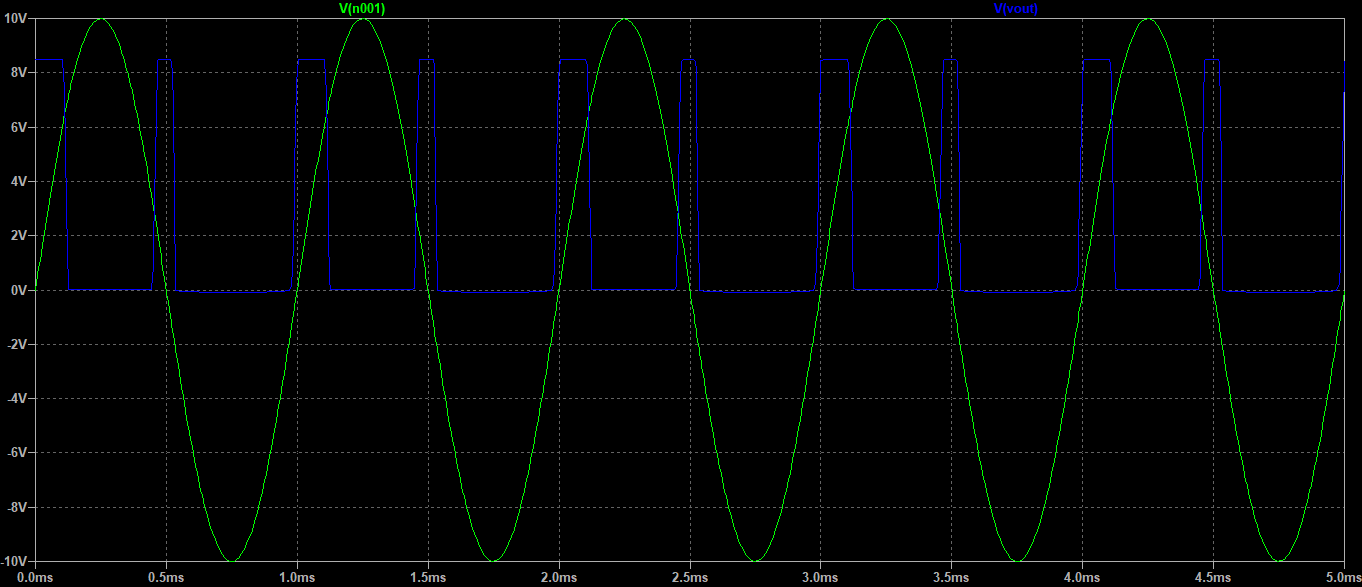
\includegraphics[width=1\textwidth]{Imagenes/comparadorVin10V.png}
	\caption{$Vo_1= f(v_{in})$ con $V_{in}$ = 10 [V] y 1[KHz] en el tiempo.}
\end{figure}
Podemos ver entonces como, a diferencia de un comparador convencional que evalúa dos voltajes de entrada y genera una señal de salida alta o baja según cuál de ellos sea mayor, un comparador con histéresis incorpora un mecanismo de memoria en el circuito. Esto implica que, una vez que la salida ha cambiado de estado, es necesario un cambio más significativo en la señal de entrada para que la salida vuelva a conmutar. Esta característica es especialmente útil en aplicaciones como la detección de niveles, el control de motores y los circuitos de disparo, ya que ayuda a evitar cambios erráticos en la salida debido a ruidos o fluctuaciones pequeñas en la señal de entrada.
\end{document}